% !TEX root = ../my-thesis.tex
%
\chapter{Introduction}
\label{sec:intro}


\begin{figure}[!b]
\centering
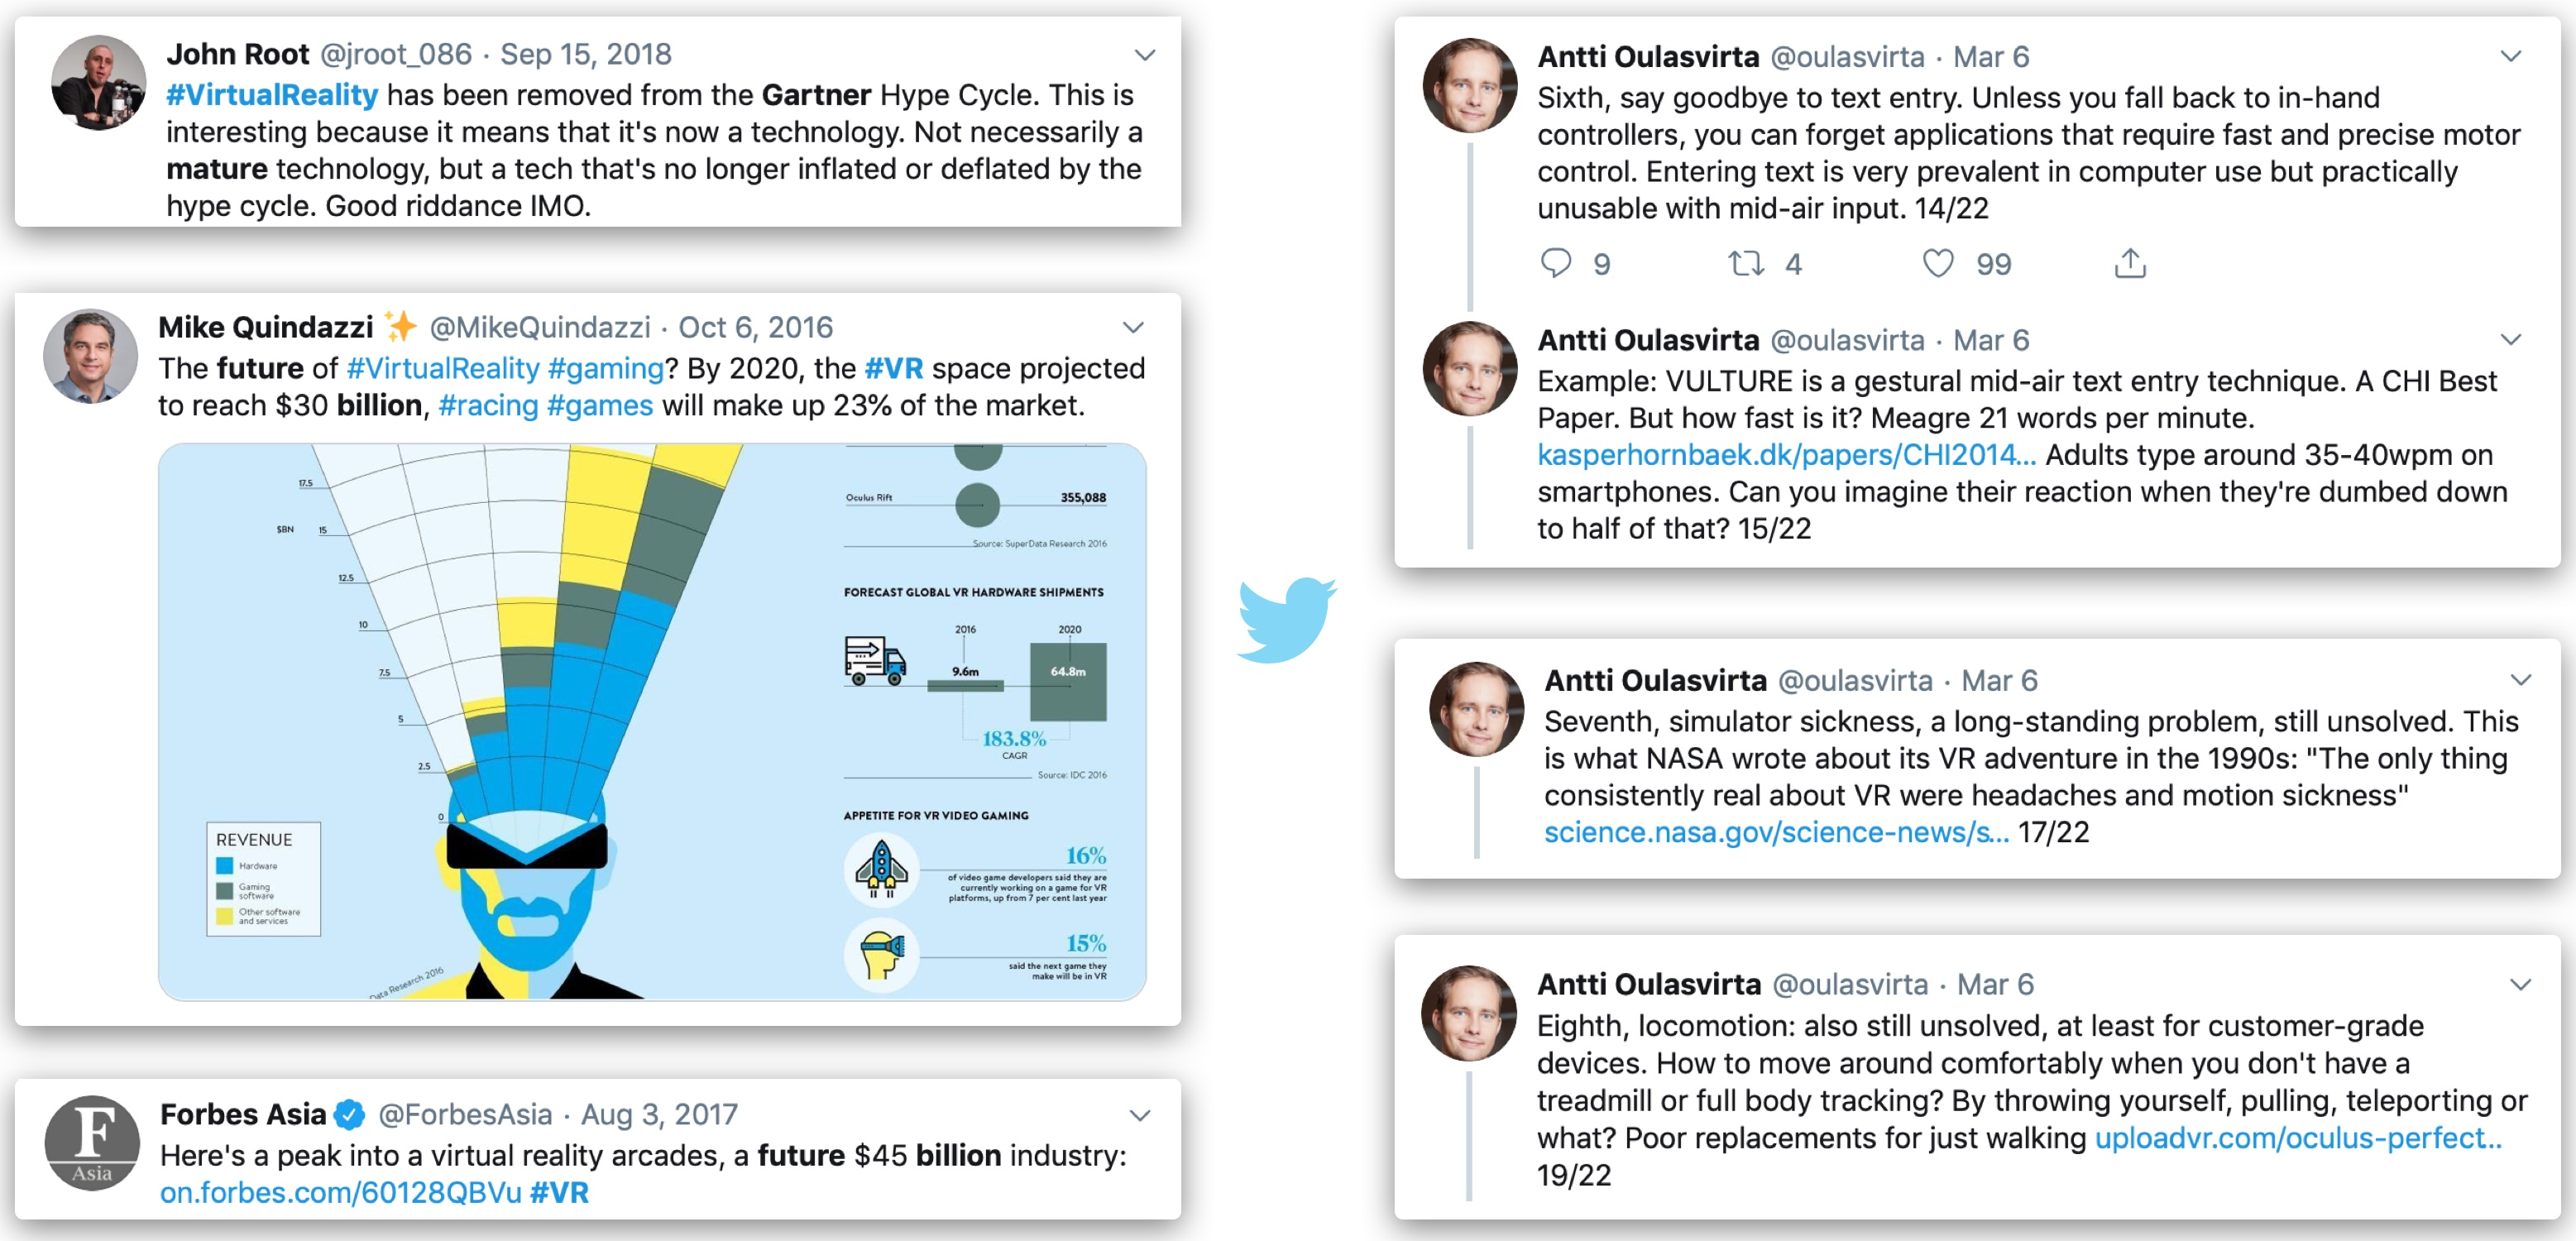
\includegraphics[width=1.0\columnwidth]{content/images/vr_tweets.jpg}
\caption{Mixed voices on Twitter regarding the present and future of virtual reality.}
\label{fig:twitter}
\end{figure}


% Annti tweeted: VR bad. is it true?
% Fin: VR isnt good, but research makes it better. Does it fix it? No.
% BUT: curiosity is human nature, and everyone in the studies loved trying vr. So, even if
% it is only an intermediate solution, we should keep it, because we are humans, after all.


Virtual Reality (VR) has taken foot in everyday life. Or didn't it? We are caught between two camps: On one hand, industry took critical leaps forward and established affordable living room VR setups. Software complanies are extending their products to VR and promise unique benefits, be it for entertainment or business purposes. On the other hand, however, researchers are getting more and more vocal (cf. \FG{fig:twitter}) regarding the omnipresent obstactles of VR that haven't changed that much in the last decades: limited locomotion, inferior interaction, or the risk of cybersickness, to name a few.

% never cap after colon when introducing a list
% cap if one or more complete sentences (On one hand,...)

% ``parentheses''


As prospective or even established researchers, we often question ourselves which impact our work in a certain area might have and whether it is ``worth it''. So, is VR doomed as some people claim, or are there good chances that our research efforts will be rewarded? Exactly that is the central question that unites the publications gathered in this thesis. As the title already reveals, we will dive into seven different VR entities to win an impression whether and how research might change the status quo of mainstream VR. The particular contributions range from foundamental techniques, such as novel locomotion approaches, to application domains, such as scientific visualization. To make the manuscript more readable, the introduction section is dedicated to answering three major questions of the reader: 
\begin{itemize}[noitemsep]
\item \textit{Why was the thesis written (and why should I read it)?}
\item \textit{What is the thesis (not) about?}
\item \textit{How is the manuscript organized?}
\end{itemize}
Note that this is a cumulative dissertation. Hence, in contrast to traditional manuscripts, the present synopsis is a high-level pointer to published works, rather than a verbose in-depth elaboration of a particular research topic. The main objectives of such a synopsis are to establish a red thread through the conducted research, to familiarize the readers with the most important outcomes, and to draw final conclusions---in our case, conclusions related to the present and future of virtual reality.






% todo: PICTURE of vr ads and anttis tweet

% ``parentheses''

\section{Motives for Revisiting VR}

One important argument among opponents of VR (research) is that the base approach of VR is not novel and has not evolved in the last decades. In fact, nearly all ``VR booms'' and associated promises failed, and many of us see no reason to believe the opposite regarding the current VR era. In the early nineties, we faced first commercial VR headsets, such as the Sega VR, and magazines predicted ``affordable VR by 1994''~\cite{engler1992affordable}. Now, more than twenty years later, VR is finally regarded as mainstream, arriving in the price range of consoles and high-end smartphones. Yet the idea remains the same: a stereo pair of images and head tracking form the base for an experience that is well-known and being studied extensively for decades---so why is it worth reconsidering it? 

As always, the devil is in the details. While there was no major invention that revolutionized VR overnight, a number of subtle advances and incremental changes---both from a technical and psychological perspective---give us enough reason to revisit VR. In order to aid clarity, such changes can be aggregated in the following categories:

\subsection{Hardware}

As it comes to technology, the most striking progress was achieved regarding the three following characteristics of VR setups: \textit{affordability}, \textit{comfort}, and \textit{features}. 

\textbf{Affordability.} In general, the price tag is not all that important in research. However, easily available HMDs created a common base for VR experiments and increased reproducibility. Thanks to default setups, such as the HTC Vive ecosystem, researchers began to share their testbed implementations and best practices, which enhanced the overall robustness and transferability of the results. 

%Furthermore, affordability helped to overcome the initial scepticism regarding the applicability of VR in industry. 


\textbf{Comfort.} In the past, wearing a heavy and chunky HMD unavoidably introduced a bias due to discomfort and limited the potential of VR. Nowadays, HMDs have an overall weight around 500 grams and can be considered at least bearable for a prolonged period of time. More importantly, the show-stopping and dangerous cable clutter finally disappeared, be it in case of all-in-one solutions, such as the Oculus Quest, or even in case of desktop VR variants, such as the HTC Vive Pro with a wireless adapter. 




% different types of hmds:
% https://www.aniwaa.com/guide/vr-ar/types-of-vr-headsets/

\textbf{Features.} Affordable and comfortable HMDs compete on the market, and this competition ensures that manufacturers have to add unique features to their products. Hence, users finally receive acceptable display resolutions and an increased, yet still narrow, field of view. Moreover, VR setups now include sophisticated and precise controllers to enhance the interaction with VR content. And, perhaps most importantly, room-scale VR paved its way into production, which allows us to utilize the most realistic locomotion technique to explore virtual environments---natural walking.







\subsection{Software}
more sophisticated software (tracking and things from research that were merged into vr)

\subsection{People}
more digital people (less cs) --most important aspect maybe


these reasons have highest impact on aspects such as locomotion, interaction, and perception, so thats why we exactly revisit it and see what we can make out of it.



% on other hand, still lots of concerns from research that say its useless, e.g., anttis tweet.

% so its polarizing, things changed and change, and thats why we need a closer look to provide some current estimates whether its holzweg wnd where the reise goes.




\section{Scope and Contentual Boundaries}
what is it about and what it is not about
- what is scope, what is outside?
- explain that there are not 7 paper, but much more
- and that we subdivide the papers in walk, touch, and see - locomotion, interaction, perception

% locomotion
% Q1: do we need an "intro" or do we start with chapter?
% Q2: how coupled are gullivr and outstanding


% interaction
% weapons, gestures, mui, inventories



to have some sort of impression, we need some big picture, and need lot of areas. time limitations so we picked representatives (things that changed most maybe). main focus on walk, see, and touch.

describe what particular questions will be answered.
- (antti) take look how to locomote in vr and present novel approaches. In particular, cybersickness and presence will be handled here (?)


- (annti) interaction in terms of gestures, haptics, representation, and software logistics


- what can we use vr for? differing perception is great


Limit to mainstream vr, no exotic setups.
many studies are with vr games as example, as one of the most important motor of such setups.


examples of what is not inside but still important: text input, multi-user.




\section{Structure of the Synopsis}

how the big picture is collected. diff areas, ranging from vr techniques (locomotion) over interaction modalities and taxonomies to perception phenomena that make vr unique and beneficial.



\section{anttis vr rant}
%%%%%%%% ANTTI TWEET
% https://twitter.com/oulasvirta/status/1103298711382380545?lang=en

Rant: Nine reasons why I don't believe in current VR/AR technology.

HoloLens, Magic Leap, and Oculus: Mind-blowing videos, and the market is estimated to explode to 200 billion by 2025 (Statista). So what's wrong?

HCI research tells why we haven't seen a killer app yet:




\subsection{the gorilla arm}

First, the gorilla arm. The videos show smiling users holding their arms up for extended periods. But that will cause shoulder pain. The Consumed Endurance model estimates that a user can hold arm up for just 90 seconds before starting to fatigue. 
% https://t.co/5MgNriW4BV

Anecdotally, when drsrinathsridha was working on a CHI paper, he could not find a comfortable posture for doing freehand gestures and had days of sore neck and arm. Well, you could try "gun slinging, but then you lose hand-to-display coupling and fall back to mouse-like input

So, either we lose hand input or we're limited to applications that that don't need more than 90 seconds of "air time". 




\subsection{hands have evolved for manipulating objects}
Second, our hands have evolved for manipulating objects, not for poking in the air. 


While vision-based tracking of hand movement has taken leaps forward, tracking of hands WITH objects hasn't. Here's a screencap from our ECCV paper from a few years back. Tracking works if you're slow and occlusions are bearable


So, it seems you can forget interactions with (arbitrary) physical objects. We're going to be designing poking-in-the-air applications for years to come. 

\subsection{poking-in-the-air is also inferior}
Third, poking-in-the-air is also inferior as a means of interaction. Mechanoreceptive feedback is specialized and important for input. We don't want to lose it. Even pressing a button or hitting a virtual ball becomes hard. 

Well, you could try 3 things: 1) forget applications where contact is needed (boo!), 2) wear gloves (clumsy, unhygienic), or 3) assume an instrumented environment. Ultrahaptics - as far as I have tried it - is too weak to replace real contact. 

Users will miss real buttons. 


\subsection{gesturing is not "natural"}
Fourth, gesturing is not "natural". There are few if any instinctual gestures. HCI research has sought for natural gestures for a decade, but found out that the gesture elicitation method artificially inflates claimed consensus: 
% https://t.co/RBslSzBSnO

So, either you forget "natural interaction", and assume that your users are willing to spend time learning new gestures, or you're stuck with simple pointing-and-pinching type gestures that users can transfer from the mobile device.



\subsection{body misalignment}
Fifth, body misalignment. This is my fav: The virtual and the physical body will never be perfectly aligned in time and space. The sensing+computation pipeline that mediates motion and display can only worsen alignment. Try petting a cat with Leap Motion. Ouch.

This is a serious issue for motor control, causing coordinate disturbance, temporal asynchrony, and poorer cue integration. Users cannot rely on their senses as they normally do when moving. Imagine tracking a bee in 3D space: Hard IRL, harder in VR


\subsection{text}
Sixth, say goodbye to text entry. Unless you fall back to in-hand controllers, you can forget applications that require fast and precise motor control. Entering text is very prevalent in computer use but practically unusable with mid-air input. 



Example: VULTURE is a gestural mid-air text entry technique. A CHI Best Paper. But how fast is it? Meagre 21 words per minute.  Adults type around 35-40wpm on smartphones. Can you imagine their reaction when they're dumbed down to half of that?
%https://t.co/Xtgf82ofGH

Well, you could design a new open-loop gesture set, like a sign language. We tried exactly that (CHI'15), predicting that you might get up to 50 WPM with simple gestures and LeapMotion-level sensing. Downside? You need to practice around 10-20 hours
% https://t.co/EtemobxzhQ


\subsection{simulator sickness}
Seventh, simulator sickness, a long-standing problem, still unsolved. This is what NASA wrote about its VR adventure in the 1990s: "The only thing consistently real about VR were headaches and motion sickness" 

ut surely we have solved motion sickness by now with better hardware? No. Depending on task, up to 56 percent of participants felt motion sickness with Oculus Rift in a recent study: 
%https://t.co/GbEr7GuXX1


\subsection{locomotion}
Eighth, locomotion: also still unsolved, at least for customer-grade devices. How to move around comfortably when you don't have a treadmill or full body tracking? By throwing yourself, pulling, teleporting or what? Poor replacements for just walking.



\subsection{fov}
Ninth, another persisting problem still with us: the narrow field of view. HoloLens had a notoriously narrow FOV "like a card deck". 

When the HMD's FOV is narrower than your (real) peripheral vision, you lose visual context. Users need to turn and glance around to orient. 

But peripheral vision is actually important in many visual tasks. NASA reported that pilots did better with traditional displays than with VR because of this. 
% https://t.co/wMKwVMCMaq


\subsection{summary}
To sum up, definite progress has been made, but the scope of today's VR/AR technology is narrow. It is locked into applications where a few seconds of waving in the air is worth the hassle of putting on an HMD.


